\begin{SCn}

\scnsectionheader{\currentname}

\scnstartsubstruct

\scnheader{Предметная область связок и отношений}
\scniselement{предметная область}
\scnsdmainclasssingle{связь}
\scnsdclass{бинарная связь;sc-коннектор;неатомарная бинарная связь;небинарная связь;неориентированная связь;ориентированная связь;отношение;класс равномощных связок;класс связок разной мощности;унарное отношение;бинарное отношение;квазибинарное отношение;тернарное отношение;небинарное отношение;ориентированное отношение;неориентированное отношение;рефлексивное отношение;антирефлексивное отношение;частично рефлексивное отношение;симметричное отношение;антисимметричное отношение;частично симметричное отношение;транзитивное отношение;антитранзитивное отношение;частично транзитивное отношение;связанное отношение;отношение порядка;отношение строгого порядка;отношение нестрогого порядка;отношение толерантности;отношение эквивалентности;ролевое отношение;числовой атрибут;неролевое отношение;неролевое бинарное отношение;арность;метаотношение;отношение декомпозиции;отношение интеграции}
\scnsdrelation{область определения*;атрибут отношения*;домен*;первый домен*;второй домен*;композиция отношений*;фактор-множество*;соответствие*;отношение соответствия*;область отправления';область прибытия’;образ';прообраз';всюду определенное соответствие*;частично определенное соответствие*;сюръективное соответствие*;несюръективное соответствие*;однозначное соответствие*;обратное соответствие*;обратимое соответствие*;неоднозначное соответствие*;инъективное соответствие*;взаимно однозначное соответствие*;множество сочетаний*;множество размещений*;множество перестановок*}

\scnheader{связь}
\scnidtf{связка sc-элементов}
\scnidtf{sc-связка}
\scnexplanation{\textbf{\textit{связь}} – множество, являющееся абстрактной моделью связи между описываемыми сущностями, которые или знаки которых являются элементами этого множества.}
\scntext{примечание}{Напомним, что все элементы множества, представленного в SC-коде, являются знаками, но описываемыми сущностями могут быть не только сущности, обозначаемые sc-элементами, но и сами эти sc-элементы.}
\scnsubdividing{бинарная связь;небинарная связь}
\scnsubdividing{неориентированная связь;ориентированная связь}

\scnheader{бинарная связь}
\scnsubdividing{sc-коннектор;неатомарная бинарная связь}
\scntext{примечание}{Данное разбиение осуществляется на основе синтаксического признака, а не семантического, поскольку каждый \textit{sc-коннектор} может быть записан в памяти при помощи семантически эквивалентной конструкции, содержащей знак самой связи и пары принадлежности, ведущие к ее элементам, уточненные, при необходимости ролевыми отношениями.}

\scnheader{sc-коннектор}
\scnidtf{атомарная бинарная связь}
\scnexplanation{Каждый \textbf{\textit{sc-коннектор}} представлен в \textit{sc-памяти} одним \textit{sc-элементом} и семантически эквивалентен конструкции, содержащей знак некоторой \textit{бинарной связи} и пары принадлежности, ведущие к элементам этой связи, уточненные, при необходимости ролевыми отношениями.

Такая конструкция может быть обозначена \textbf{\textit{sc-коннектором}} только в случае, когда роли компонентов соответствующей бинарной связи указываются только при помощи \textit{числовых атрибутов 1’} и \textit{2’} или не уточняются вообще.}

\scnheader{неатомарная бинарная связь}
\scnexplanation{\textbf{\textit{неатомарная бинарная связь}} – \textit{бинарная связь}, роли компонентов которой не могут быть заданы только при помощи \textit{ролевых отношений 1'} и \textit{2'}, или не заданы совсем, а требуют дополнительного уточнения при помощи более частных ролевых отношений.}

\scnheader{небинарная связь}
\scnexplanation{\textbf{\textit{небинарная связь}} – связь, имеющая больше двух элементов.}

\scnheader{неориентированная связь}
\scnsuperset{неориентированное множество}
\scnexplanation{\textbf{\textit{неориентированная связь}} – связь, все элементы которой имеют одинаковые роли (при этом соответствующее ролевое отношение, как правило, явно не указывается).}

\scnheader{ориентированная связь}
\scnsuperset{ориентированное множество}
\scnexplanation{\textbf{\textit{ориентированная связь}} – связь, в которой с помощью ролевых отношений, указываются роли компонентов этой связи.}

\scnheader{отношение}
\scnidtf{класс связей}
\scnidtf{класс sc-связок}
\scnidtf{множество отношений}
\scnidtf{Множество всевозможных отношений}
\scntext{определение}{\textbf{\textit{отношение}}, \textit{заданное на множестве M} – это подмножество \textit{декартового произведения} этого множества самого на себя некоторое количество раз.

В более широком смысле \textbf{\textit{отношение}} – это математическая структура, которая формально определяет свойства различных объектов и их взаимосвязи.}
\scnsubdividing{класс равномощных связок;класс связок разной мощности}
\scnsubdividing{бинарное отношение;небинарное отношение}
\scnsubdividing{ориентированное отношение;неориентированное отношение}
\scnsubdividing{ролевое отношение;неролевое отношение}

\scnheader{класс равномощных связок}
\scnidtf{класс связок фиксированной арности}
\scnidtf{отношение, обладающее свойством арности}
\scnsuperset{унарное отношение}
\scnsuperset{бинарное отношение}
\scnsuperset{тернарное отношение}
\scntext{определение}{\textbf{\textit{класс равномощных связок}} – класс связок, имеющих одинаковую мощность.}

\scnheader{класс связок разной мощности}
\scnidtf{отношение нефиксированной арности}
\scnsubset{небинарное отношение}
\scntext{определение}{\textbf{\textit{класс связок разной мощности}} – класс связок, имеющих разную мощность.}

\scnheader{унарное отношение}
\scnidtf{отношение арности один}
\scnidtf{одноместное отношение}
\scnidtf{множество синглетонов}
\scntext{определение}{\textbf{\textit{унарное отношение}} – это множество таких отношений на множестве M, являющихся любым подмножеством множества M.}

\scnheader{бинарное отношение}
\scnidtf{отношение арности два}
\scnidtf{двухместное отношение}
\scnsuperset{квазибинарное отношение}
\scnsuperset{отношение порядка}
\scnsuperset{отношение толерантности}
\scnsubdividing{рефлексивное отношение;антирефлексивное отношение;частично рефлексивное отношение}
\scnsubdividing{симметричное отношение;антисимметричное отношение;частично симметричное отношение}
\scnsubdividing{транзитивное отношение;антитранзитивное отношение;частично транзитивное отношение}
\scnsubdividing{ролевое отношение;неролевое бинарное отношение}
\scntext{определение}{\textbf{\textit{бинарное отношение}} – это множество таких отношений на множестве \textbf{\textit{M}}, являющихся подмножеством \textit{декартова произведения} множества \textbf{\textit{M}}.\\
Если \textbf{\textit{бинарное отношение R}} задано на \textit{множестве} \textbf{\textit{М}} и два элемента этого множества \textbf{\textit{a}} и \textbf{\textit{b}} связаны данным отношением, то будем обозначать такую связь как \textbf{\textit{aRb}}.}

\scnheader{квазибинарное отношение}
\scnexplanation{\textbf{\textit{квазибинарное отношение}} – множество ориентированных пар, первые компоненты которых являются связками.\\
Таким образом, \textit{sc-дуги}, принадлежащие \textbf{\textit{квазибинарным отношениям}}, всегда выходят из связок.}
\scntext{sc-утверждение}{В область определения квазибинарного отношения будем включать:
\begin{scnitemize}
    \item вторые компоненты ориентированных пар, принадлежащих этому отношению;
    \item элементы первых компонентов ориентированных пар, принадлежащих этому отношению;
    \item других элементов область определения квазибинарного отношения не содержит.
\end{scnitemize}
}

\scnheader{тернарное отношение}
\scnidtf{отношение арности три}
\scnidtf{трехместное отношение}
\scnexplanation{\textbf{\textit{тернарное отношение}} – это множество отношений, связывающих между собой три элемента.}

\scnheader{небинарное отношение}
\scnexplanation{\textbf{\textit{небинарное отношение}} – это множество отношений, хотя бы одна из связок каждого из которых имеет значение мощности больше двух.}

\scnheader{ориентированное отношение}
\scntext{определение}{\textbf{\textit{ориентированное отношение}} – это множество таких отношений, каждая связка которых является ориентированным множеством.}

\scnheader{неориентированное отношение}
\scntext{определение}{\textbf{\textit{неориентированное отношение}} – это множество таких отношений, каждая связка которых является неориентированным множеством.}

\scnheader{рефлексивное отношение}
\scntext{определение}{\textbf{\textit{рефлексивное отношение}} – это \textit{бинарное отношение}, любая пара которого есть канторовское множество.}

\scnheader{антирефлексивное отношение}
\scntext{определение}{\textbf{\textit{антирефлексивное отношение R}} на \textit{множестве} \textbf{\textit{A}} – это \textit{бинарное отношение}, в котором все элементы множества \textbf{\textit{A}} не находятся в отношении \textbf{\textit{R}} к самому себе.}

\scnheader{частично рефлексивное отношение}
\scntext{определение}{\textbf{\textit{частично рефлексивное отношение R}} на \textit{множестве} \textbf{\textit{A}} – это \textit{бинарное отношение},  в котором хотя бы один (но не все) элемент множества \textbf{\textit{A}} находится в отношении \textbf{\textit{R}} к самому себе.}

\scnheader{симметричное отношение}
\scntext{определение}{\textbf{\textit{симметричное отношение R}} на \textit{множестве} \textbf{\textit{A}} – это \textit{бинарное отношение}, в котором для каждой пары элементов \textbf{\textit{а}} и \textbf{\textit{b}} этого множества выполнение отношения \textbf{\textit{aRb}} влечёт выполнение \textbf{\textit{bRa}}.}

\scnheader{антисимметричное отношение}
\scntext{определение}{\textbf{\textit{антисимметричное отношение R}} на \textit{множестве} \textbf{\textit{A}} – это \textit{бинарное отношение}, в котором для каждой пары элементов \textbf{\textit{а}} и \textbf{\textit{b}} этого множества выполнение отношений \textbf{\textit{aRb}} и \textbf{\textit{bRa}} влечёт равенство \textbf{\textit{a}} и \textbf{\textit{b}}.}

\scnheader{частично симметричное отношение}
\scntext{определение}{\textbf{\textit{частично симметричное отношение R}} на \textit{множестве} \textbf{\textit{A}} – это \textit{бинарное отношение}, в котором для каждой пары элементов \textbf{\textit{а}} и \textbf{\textit{b}} (но не для всех таких пар) этого множества выполнение отношения \textbf{\textit{aRb}} влечёт выполнение \textbf{\textit{bRa}}.}

\scnheader{транзитивное отношение}
\scntext{определение}{\textbf{\textit{транзитивное отношение R}} на \textit{множестве} \textbf{\textit{A}} – это \textit{бинарное отношение}, в котором для любых трёх элементов этого множества \textbf{\textit{a, b, c}} выполнение отношений \textbf{\textit{aRb}} и \textbf{\textit{bRc}} влечёт выполнение отношения \textbf{\textit{aRc}}.}

\scnheader{антитранзитивное отношение}
\scntext{определение}{\textbf{\textit{антитранзитивное отношение R}} на \textit{множестве} \textbf{\textit{A}} – это \textit{бинарное отношение}, в котором для любых трёх элементов этого множества \textbf{\textit{a, b, c}} выполнение отношений \textbf{\textit{aRb}} и \textbf{\textit{bRc}} не влечёт выполнение отношения \textbf{\textit{aRc}}.}

\scnheader{частично транзитивное отношение}
\scntext{определение}{\textbf{\textit{частично транзитивное отношение R}} на \textit{множестве} \textbf{\textit{A}} – это \textit{бинарное отношение}, в котором для каждых трёх элементов этого множества \textbf{\textit{a, b, c}} (но не для всех таких троек) выполнение отношений \textbf{\textit{aRb}} и \textbf{\textit{bRc}} влечёт выполнение отношения \textbf{\textit{aRc}}.}

\scnheader{связанное отношение}
\scnsubset{бинарное отношение}
\scntext{определение}{\textbf{\textit{связанное отношение R}} на \textit{множестве} \textbf{\textit{A}} – это \textit{бинарное отношение}, в котором для каждой пары элементов \textbf{\textit{а}} и \textbf{\textit{b}} этого множества выполняется одно из двух отношений: \textbf{\textit{aRb}} или \textbf{\textit{bRa}}.}

\scnheader{отношение порядка}
\scnsubdividing{отношение строгого порядка;отношение нестрогого порядка}
\scntext{определение}{\textbf{\textit{отношение порядка}} – это \textit{бинарное отношение}, обладающее свойством транзитивности и антисимметричности.}

\scnheader{отношение строгого порядка}
\scntext{определение}{\textbf{\textit{отношение строгого порядка}} – это \textit{отношение порядка}, обладающее свойством антирефлексивности.}

\scnheader{отношение нестрогого порядка}
\scntext{определение}{\textbf{\textit{отношение нестрогого порядка}} – это \textit{отношение порядка}, обладающее свойством рефлексивности.}

\scnheader{отношение толерантности}
\scntext{определение}{\textbf{\textit{отношение толерантности}} – это \textit{бинарное отношение}, принадлежащее классам \textit{симметричное отношение} и \textit{рефлексивное отношение}.}

\scnheader{отношение эквивалентности}
\scnidtf{максимальное семейство отношений эквивалентности}
\scnsubset{отношение толерантности}
\scntext{определение}{\textbf{\textit{отношение эквивалентности}} – это \textit{отношение толерантности}, принадлежащее классу \textit{транзитивных отношений}}
\scntext{примечание}{Каждое отношение эквивалентности уточняет то, что мы считаем эквивалентными сущностями, т.е. то, на какие сходства этих сущностей мы обращаем внимание и какие их отличия мы игнорируем (не учитываем).}

\scnheader{ролевое отношение}
\scnidtf{атрибут}
\scnidtf{атрибутивное отношение}
\scnidtf{отношение, которое задает роль элементов в рамках некоторого множества}
\scnidtf{отношение, являющееся подмножеством отношения принадлежности}
\scnrelto{семейство подмножеств}{принадлежность*}
\scnsubset{бинарное отношение}
\scnsuperset{числовой атрибут}
\scnexplanation{\textbf{\textit{ролевое отношение}} – это отношение, являющееся подмножеством отношения принадлежности.}
\scntext{правило идентификации экземпляров}{В конце каждого \textit{идентификатора}, соответствующего экземплярам класса \textbf{\textit{ролевое отношение}}, не являющегося системным, ставится знак «'».

Например:\\
\textit{ключевой экземпляр’}

Из-за ограничений в разрешенном алфавите символов, в системном идентификаторе не может быть использовать знак «'», поэтому в начале каждого \textit{системного идентификатора}, соответствующего экземплярам класса \textbf{\textit{ролевое отношение}} ставится префикс «rrel\_».

Например:\\
\textit{rrel\_key\_sc\_element}}

\scnheader{числовой атрибут}
\scnidtf{порядковый номер}
\scnidtf{номер компонента ориентированной связки}
\scnhaselement{1’; 2’; 3’; 4’; 5’; 6’; 7’; 8’; 9’; 10’}
\scnexplanation{\textbf{\textit{числовой атрибут}} – \textit{ролевое отношение}, задающее порядковый номер элемента некоторой ориентированной связки, не уточняя при этом семантику такой принадлежности. Во многих случаях бывает достаточно использовать числовые атрибуты, чтобы различать компоненты связки, семантика каждого из которых дополнительно оговаривается, например, при определении отношения, которому данная связка принадлежит.}

\scnheader{неролевое отношение}
\scnsubdividing{небинарное отношение;неролевое бинарное отношение}
\scnexplanation{\textbf{\textit{неролевое отношение}} – отношение, не являющееся подмножеством отношения принадлежности.}
\scntext{правило идентификации экземпляров}{В конце каждого \textit{идентификатора}, соответствующего экземплярам класса \textbf{\textit{неролевое отношение}}, не являющегося системным, ставится знак «*».

Например:\\
\textit{включение*}

Из-за ограничений в разрешенном алфавите символов, в системном идентификаторе не может быть использовать знак «*», поэтому в начале каждого \textit{системного идентификатора}, соответствующего экземплярам класса \textbf{\textit{неролевое отношение}} ставится префикс «nrel\_».

Например:\\
\textit{nrel\_inclusion}}

\scnheader{неролевое бинарное отношение}
\scnexplanation{\textbf{\textit{неролевое бинарное отношение}} – \textit{бинарное отношение}, не являющееся \textit{ролевым отношением}.}

\scnheader{арность}
\scnidtf{арность отношения}
\scniselement{параметр}
\scnexplanation{\textbf{\textit{арность}} – это параметр, каждый элемент которого представляет собой класс \textit{отношений}, каждая связка которых имеет одинаковую \textit{мощность}. Значение данного \textit{параметра} совпадает со значением \textit{мощности} каждой из таких связок.}
\scnrelfrom{описание типичного экземпляра}{
\scnfilescg{figures/sd_relations/arity.png}}


\scnheader{область определения*}
\scnidtf{область определения отношения*}
\scniselement{бинарное отношение}
\scnexplanation{\textbf{\textit{область определения*}} – это \textit{бинарное отношение}, связывающее отношение со множеством, являющимся его областью определения.

Областью определения отношения будем называть результат теоретико-множественного объединения всех связок этого отношения, или, другими словами, результат теоретико-множественного объединения всех множеств, являющихся доменами данного отношения.}
\scnrelfrom{описание типичного экземпляра}{
\scnfilescg{figures/sd_relations/domain.png}}

\scnheader{атрибут отношения*}
\scnidtf{ролевой атрибут, используемый в связках заданного отношения*}
\scniselement{бинарное отношение}
\scnexplanation{\textbf{\textit{атрибут отношения*}} – это \textit{бинарное отношение}, связывающее заданное отношение с \textit{ролевым отношением}, используемым в данном отношении для уточнения роли того или иного элемента связок данного отношения.}
\scnrelfrom{описание типичного экземпляра}{
\scnfilescg{figures/sd_relations/relationshipAttribute.png}}


\scnheader{домен*}
\scnidtf{домен отношения по заданному атрибуту*}
\scniselement{бинарное отношение}
\scnexplanation{\textbf{\textit{домен*}} – это \textit{бинарное отношение}, связывающее связку отношения \textit{атрибут отношения*} со множеством, являющимся доменом заданного отношения по заданному атрибуту. Множество \textbf{\textit{di}} является доменом отношения \textbf{\textit{ri}} по атрибуту \textbf{\textit{ai}} в том и только том случае, если элементами этого множества являются все те и только те элементы связок отношения \textbf{\textit{ri}}, которые имеют в рамках этих связок атрибут \textbf{\textit{ai}}.}
\scnrelfrom{описание типичного экземпляра}{
\scnfilescg{figures/sd_relations/domen.png}}


\scnheader{первый домен*}
\scniselement{бинарное отношение}
\scntext{определение}{\textbf{\textit{первый домен*}} – это \textit{бинарное отношение}, связывающее отношение с множеством, являющимся доменом по атрибуту \textbf{\textit {1'}} данного отношения.}
\scnrelfrom{описание типичного экземпляра}{
\scnfilescg{figures/sd_relations/firstDomain.png}}

\scnheader{второй домен*}
\scniselement{бинарное отношение}
\scntext{определение}{\textbf{\textit{второй домен*}} – это \textit{бинарное отношение}, связывающее отношение с множеством, являющимся доменом по атрибуту \textbf{\textit{2'}} данного отношения.}
\scnrelfrom{описание типичного экземпляра}{
\scnfilescg{figures/sd_relations/secondDomain.png}}

\scnheader{композиция отношений*}
\scniselement{квазибинарное отношение}
\scntext{определение}{\textbf{\textit{композиция отношений*}} – это \textit{квазибинарное отношение}, связывающее два бинарных отношения с отношением, являющимся их композицией. Под композицией бинарных отношений \textbf{\textit{R}} и \textbf{\textit{S}} будем понимать множество $\{(x, y) | \exists z(xSz \wedge zRy)\}$}
\scnrelfrom{описание типичного экземпляра}{
\scnfilescg{figures/sd_relations/relationshipComposition.png}}

\scnheader{фактор-множество*}
\scnidtf{быть фактор-множеством*}
\scnidtf{множество всевозможных максимальных множеств из попарно эквивалентных элементов*}
\scnidtf{множество всевозможных классов эквивалентности для заданного отношения эквивалентности*}
\scniselement{бинарное отношение}
\scntext{определение}{\textbf{\textit{фактор множество*}} - это бинарное ориентированное отношение, каждая связка которого связывает некоторое отношение эквивалентности со множеством всех соответствующих этому отношению классов эквивалентности. Каждый такой класс представляет собой максимальное множество сущностей, каждая пара которых принадлежит указанному выше отношению эквивалентности.}
\scnrelfrom{описание типичного экземпляра}{
\scnfilescg{figures/sd_relations/factor_set.png}}

\scnheader{метаотношение}
\scntext{определение}{метаотношение - это \textit{отношение}, в каждой связке которого есть по крайней мере один компонент, являющийся знаком некоторого \textit{отношения}.}

\scnheader{отношение декомпозиции}
\scnhaselement{разбиение*}
\scnhaselement{декомпозиция раздела*}
\scnhaselement{декомпозиция абстрактного объекта*}

\scnheader{отношение интеграции}
\scnhaselement{объединение*}

\scnheader{соответствие*}
\scnidtf{наличие соответствия*}
\scniselement{бинарное отношение}
\scnsubdividing{соответствие между непересекающимися множествами*;соответствие между строго пересекающимися множествами*;соответствие, область отправления и область прибытия которого совпадают*}
\scnsubdividing{всюду определенное соответствие*;частично определенное соответствие*}
\scnsubdividing{сюръекция*;несюръективное соответствие*}
\scnsubdividing{однозначное соответствие*;неоднозначное соответствие*}
\scntext{определение}{\textbf{\textit{соответствие*}} – \textit{бинарное отношение}, заданное на множествах и задающее наличие отношения, в котором участвуют только элементы этих множеств.}
\scnrelfrom{описание типичного экземпляра}{
\scnfilescg{figures/sd_relations/conformity.png}}

\scnheader{отношение соответствия*}
\scniselement{бинарное отношение}
\scntext{определение}{\textbf{\textit{отношение соответствия*}} – \textit{бинарное отношение}, связывающее ориентированную пару множеств, на которых задано \textit{соответствие*} и некоторое подмножество \textit{декартова произведения*} этих \textit{множеств}.}
\scnrelfrom{описание типичного экземпляра}{
\scnfilescg{figures/sd_relations/relationshipConformity.png}}

\scnheader{область отправления'}
\scnidtf{область отправления соответствия’}
\scnidtf{область определения соответствия’}
\scnidtf{первый компонент пары в отношении соответствия’}
\scniselement{ролевое отношение}
\scntext{определение}{\textbf{\textit{область отправления'}} – \textit{ролевое отношение}, указывающее на первый компонент пары в рамках отношения \textit{соответствие*}.}
\scnrelfrom{описание типичного экземпляра}{
\scnfilescg{figures/sd_relations/departureArea.png}}

\scnheader{область прибытия’}
\scnidtf{область прибытия соответствия'}
\scnidtf{область значений соответствия'}
\scniselement{ролевое отношение}
\scntext{определение}{\textbf{\textit{область прибытия’}} – \textit{ролевое отношение}, указывающее на второй компонент пары в рамках отношения \textit{соответствие*}.}
\scnrelfrom{описание типичного экземпляра}{
\scnfilescg{figures/sd_relations/arrivalArea.png}}

\scnheader{образ'}
\scnidtf{образ соответствия’}
\scniselement{ролевое отношение}
\scntext{определение}{\textbf{\textit{образ'}} – \textit{ролевое отношение}, указывающее на второй компонент каждой пары в рамках множества пар, которое является вторым компонентом \textit{отношения соответствия*}.}
\scnrelfrom{описание типичного экземпляра}{
\scnfilescg{figures/sd_relations/form.png}}

\scnheader{прообраз'}
\scnidtf{прообраз соответствия’}
\scniselement{ролевое отношение}
\scntext{определение}{\textbf{\textit{прообраз'}} – \textit{ролевое отношение}, указывающее на первый компонент каждой пары в рамках множества пар, которое является первым компонентом \textit{отношения соответствия*}.}
\scnrelfrom{описание типичного экземпляра}{
\scnfilescg{figures/sd_relations/prototype.png}}

\scnheader{всюду определенное соответствие*}
\scnidtf{полное соответствие*}
\scnidtf{наличие всюду определенного соответствия*}
\scntext{определение}{\textbf{\textit{всюду определенное соответствие*}} – это \textit{соответствие*}, при котором существует \textit{образ’} для каждого элемента \textit{области отправления'} данного \textit{соответствия*}.}
\scnrelfrom{описание типичного экземпляра}{
\scnfilescg{figures/sd_relations/surjection.png}}
\scnrelfrom{изображение}{
\scnfileimage{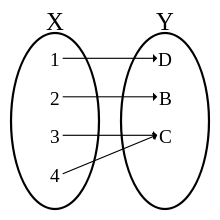
\includegraphics[width=0.5\linewidth]{figures/sd_relations/surjection2.png}}}


\scnheader{частично определенное соответствие*}
\scnidtf{наличие частично определенного соответствия*}
\scntext{определение}{\textbf{\textit{частично определенное соответствие*}} – это \textit{соответствие*}, при котором существует \textit{образ’} для некоторых, но не всех элементов \textit{области отправления'} данного \textit{соответствия*}.}
\scnrelfrom{описание типичного экземпляра}{
\scnfilescg{figures/sd_relations/partiallyDefinedConformity.png}}
\scnrelfrom{изображение}{
\scnfileimage{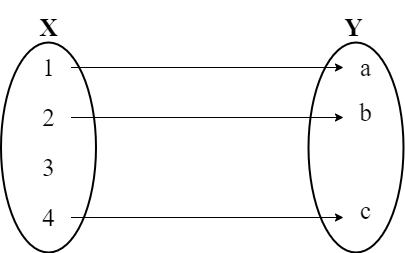
\includegraphics[width=0.5\linewidth]{figures/sd_relations/partiallySurjection.png}}}


\scnheader{сюръективное соответствие*}
\scnidtf{наличие сюръективного соответствия*}
\scnidtf{сюръекция*}
\scntext{определение}{\textbf{\textit{сюръективное соответствие*}} – это \textit{соответствие*}, при котором существует \textit{прообраз’} для каждого элемента \textit{области прибытия'} данного \textit{соответствия*}.}
\scnrelfrom{описание типичного экземпляра}{
\scnfilescg{figures/sd_relations/surjectiveConformity.png}}
\scnrelfrom{изображение}{
\scnfileimage{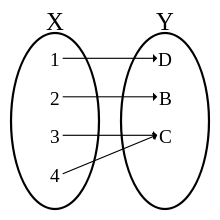
\includegraphics[width=0.5\linewidth]{figures/sd_relations/surjectiveConformity2.png}}}

\scnheader{несюръективное соответствие*}
\scnidtf{наличие несюръективного соответствия*}
\scntext{определение}{\textbf{\textit{несюръективное соответствие*}} – это \textit{соответствие*}, при котором не для каждого элемента \textit{области прибытия'} данного \textit{соответствия*} существует \textit{прообраз’}.}
\scnrelfrom{описание типичного экземпляра}{
\scnfilescg{figures/sd_relations/nonSurjectiveConformity.png}}
\scnrelfrom{изображение}{
\scnfileimage{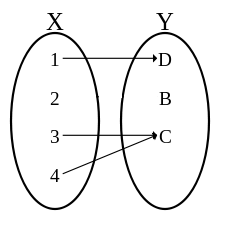
\includegraphics[width=0.5\linewidth]{figures/sd_relations/nonSurjectiveConformity2.png}}}

\scnheader{однозначное соответствие*}
\scnidtf{наличие однозначного соответствия*}
\scnidtf{функциональное соответветствие*}
\scnidtf{функция*}
\scntext{определение}{\textbf{\textit{однозначное соответствие*}} – это \textit{соответствие*}, при котором каждому элементу из \textit{области отправления'} соответствия ставится не более, чем один элемент из \textit{области прибытия’} соответствия.}
\scnrelfrom{описание типичного экземпляра}{
\scnfilescg{figures/sd_relations/singleConformity.png}}
\scnrelfrom{изображение}{
\scnfileimage{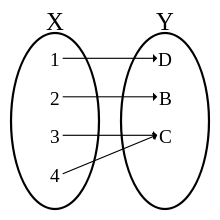
\includegraphics[width=0.5\linewidth]{figures/sd_relations/singleConformity2.png}}}

\scnheader{обратное соответствие*}
\scniselement{бинарное отношение}
\scnrelfrom{область определения}{соответствие*}
\scntext{определение}{\textbf{\textit{обратное соответствие*}} – \textit{бинарное отношение}, связывающее два \textit{соответствия*}, при этом выполняются следующие условия:
\begin{scnitemize}
    \item \textit{область отправления’} первого соответствия является \textit{областью прибытия'} второго;
    \item \textit{область прибытия’} первого соответствия является \textit{областью отправления'} второго;
    \item для каждой пары, входящей в состав отношения первого соответствия, существует пара, входящая в состав отношения второго соответствия, при этом \textit{образ’} и \textit{прообраз'} в рамках первой указанной пары являются соответственно \textit{прообразом'} и \textit{образом’} в рамках второй.
\end{scnitemize}
}

\scnheader{обратимое соответствие*}
\scnsubset{однозначное соответствие*}
\scntext{определение}{\textbf{\textit{обратимое соответствие*}} – такое \textit{однозначное соответствие*}, для которого \textit{обратное соответствие*} также является \textit{однозначным соответствием*}.}

\scnheader{неоднозначное соответствие*}
\scntext{определение}{\textbf{\textit{неоднозначное соответствие*}} – это \textit{соответствие*}, при котором хотя бы одному элементу из \textit{области отправления’} соответствия ставится более, чем один элемент из \textit{области прибытия'} соответствия.}
\scnrelfrom{описание типичного экземпляра}{
\scnfilescg{figures/sd_relations/nonSingleConformity.png}}
\scnrelfrom{изображение}{
\scnfileimage{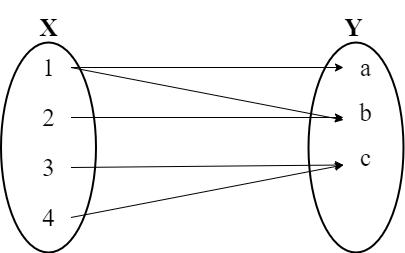
\includegraphics[width=0.5\linewidth]{figures/sd_relations/nonSingleConformity2.png}}}

\scnheader{инъективное соответствие*}
\scnidtf{инъекция*}
\scnsubset{однозначное соответствие*}
\scntext{определение}{\textbf{\textit{инъективное соответствие*}} – это \textit{соответствие*}, при котором разным элементам из \textit{области отправления’} соответствия всегда соответствуют разные элементы из \textit{области прибытия'} соответствия и наоборот.}
\scnrelfrom{описание типичного экземпляра}{
\scnfilescg{figures/sd_relations/injectiveConformity.png}}
\scnrelfrom{изображение}{
\scnfileimage{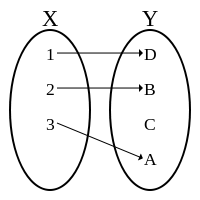
\includegraphics[width=0.5\linewidth]{figures/sd_relations/injectiveConformity2.png}}}

\scnheader{взаимно однозначное соответствие*}
\scnidtf{биекция*}
\scnsubset{всюду определенное соответствие*}
\scnsubset{сюръективное соответствие*}
\scnsubset{инъективное соответствие*}
\scntext{определение}{\textbf{\textit{взаимно однозначное соответствие*}} – это \textit{инъективное соответствие*}, являющееся всюду определенным и сюръективным.}
\scnrelfrom{описание типичного экземпляра}{
\scnfilescg{figures/sd_relations/bijectiveConformity.png}}
\scnrelfrom{изображение}{
\scnfileimage{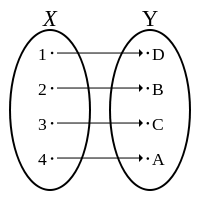
\includegraphics[width=0.5\linewidth]{figures/sd_relations/bijectiveConformity2.png}}}


\scnheader{множество сочетаний*}
\scnidtf{множество всевозможных сочетаний*}
\scnidtf{множество всевозможных сочетаний заданной арности из элементов заданного множества*}
\scnidtf{множество всех неориентированных связок заданной арности*}
\scnidtf{множество всех подмножеств заданной мощности*}
\scnidtf{семейство всевозможных сочетаний*}
\scntext{определение}{\textbf{\textit{множество сочетаний*}} - \textit{отношение}, связывающее некоторое множество и семейство всевозможных множеств, имеющих значение мощности, меньше либо равное мощности исходного множества и состоящих из тех же элементов, что и это множество.}
\scntext{утверждение}{Мощность \textbf{\textit{множества сочетаний*}} может быть вычислена как n!/(k!(n-k)!), где \textbf{\textit{n}} – мощность исходного множества, \textbf{\textit{k}} – мощность элементов множества сочетаний.}
\scnrelfrom{описание типичного экземпляра}{
\scnfilescg{figures/sd_relations/setsOfCombinations.png}
\scntext{комментарий}{Для Множества \textbf{\textit{Si}} представлено множество сочетаний по 2 элемента.}}

\scnheader{множество размещений*}
\scntext{определение}{\textbf{\textit{множество размещений*}} - \textit{отношение}, связывающее некоторое множество и семейство всевозможных кортежей, имеющих значение мощности, меньше либо равное мощности исходного множества и состоящих из тех же элементов, что и это множество.}
\scntext{утверждение}{Мощность \textbf{\textit{множества сочетаний*}} может быть вычислена как n!/(n-k)!, где \textbf{\textit{n}} – мощность исходного множества, \textbf{\textit{k}} – мощность элементов множества сочетаний.}
\scnrelfrom{описание типичного экземпляра}{
\scnfilescg{figures/sd_relations/setsOfPlacements.png}
\scntext{комментарий}{Для Множества \textbf{\textit{Si}} представлено множество размещений по 2 элемента.}}

\scnheader{множество перестановок*}
\scnsubset{множество размещений*}
\scntext{определение}{\textbf{\textit{множество перестановок*}} - \textit{отношение}, связывающее некоторое множество и семейство всевозможных кортежей, равномощных исходному множеству и состоящих из тех же элементов, что и это множество.}
\scntext{утверждение}{Мощность \textbf{\textit{множества перестановок*}} может быть вычислена как n!, где \textbf{\textit{n}} – мощность исходного множества.}
\scnrelfrom{описание типичного экземпляра}{
\scnfilescg{figures/sd_relations/setsOfPermutations.png}
\scntext{комментарий}{Для Множества \textbf{\textit{Si}} представлено его множество перестановок.}}
\scnendstruct

\end{SCn}